\documentclass[11pt,a4paper]{article}
\usepackage[T1]{fontenc}
\usepackage[utf8]{inputenc}
\usepackage{lmodern}
\usepackage{amsmath,amssymb,amsthm,mathtools,mathrsfs}
\usepackage{graphicx,float,xcolor,multicol}
\usepackage[shortlabels]{enumitem}
\usepackage[margin=27mm]{geometry}
\usepackage{microtype,needspace,placeins}
\usepackage{tikz,tikz-cd}
\usetikzlibrary{arrows.meta,calc,positioning,patterns,decorations.pathreplacing}
\usepackage[colorlinks=true,linkcolor=teal,urlcolor=teal,citecolor=teal]{hyperref}
\setlength{\parindent}{0pt}
\setlength{\parskip}{.6em}
\setcounter{secnumdepth}{0}
\allowdisplaybreaks
\raggedbottom
\providecommand{\cross}{\times}
\DeclareUnicodeCharacter{2020}{\ensuremath{\dagger}}
\DeclareMathOperator{\supp}{supp}
\DeclareMathOperator*{\esssup}{ess\,sup}
\providecommand{\chapter}{\section}
\newenvironment{tool}[2]{\subsection*{Tool #1 --- #2}}{}
\newcommand{\ToolRef}[1]{Tool #1}
\newcommand{\FigureTag}[2]{\textit{Figure #1}}
\newcommand{\Result}[1]{\subsection*{#1}}
\newcommand{\Application}[1]{\subsubsection*{Application\if\relax\detokenize{#1}\relax\else\space--- #1\fi}}
\newcommand{\ProofHeading}{\par\textit{Proof.}\space}
\newcommand{\ProofOf}[1]{\par\textit{Proof of #1.}\space}
\newcommand{\RemarkHeading}{\par\textbf{Remark.}\space}
\newcommand{\NoteHeading}{\par\textbf{Note.}\space}
\newcommand{\ExerciseHeading}{\par\textbf{Exercise.}\space}

% Rendering support only; mathematical text is in each independent post.
\usepackage{booktabs,array,longtable}
\definecolor{HandoutBlue}{HTML}{2F6690}
\definecolor{HandoutNavy}{HTML}{17365D}
\newtheorem{theorem}{Theorem}
\newtheorem{lemma}[theorem]{Lemma}
\newtheorem{proposition}[theorem]{Proposition}
\newtheorem{corollary}[theorem]{Corollary}
\newtheorem{conjecture}[theorem]{Conjecture}
\newtheorem{definition}{Definition}
\newtheorem{example}{Example}
\newtheorem{namedtoolcounter}{Tool}
\newenvironment{namedtool}[1]{\begin{namedtoolcounter}[#1]}{\end{namedtoolcounter}}
\newtheorem*{claim}{Claim}
\newtheorem*{remark}{Remark}
\newtheorem*{exercise}{Exercise}
\newtheorem*{question}{Question}
\newtheorem*{observation}{Observation}
\newcommand{\SourceChapter}[2]{\section*{#2}}
\newcommand{\Lecture}[2]{\section*{Lecture #1: #2}}
\newcommand{\unclear}[1]{\textit{[unclear: #1]}}
\newcommand{\sourcegap}{\textit{[unfinished in the source]}}
\DeclareMathOperator{\dist}{dist}
\DeclareMathOperator{\id}{id}
\DeclareMathOperator{\Hol}{Hol}
\DeclareMathOperator{\Per}{Per}
\DeclareMathOperator{\Fix}{Fix}
\DeclareMathOperator{\diam}{diam}
\DeclareMathOperator{\Var}{Var}
\DeclareMathOperator{\Leb}{Leb}
\DeclareMathOperator{\Hom}{Hom}
\DeclareMathOperator{\End}{End}
\DeclareMathOperator{\Ann}{Ann}
\DeclareMathOperator{\Spec}{Spec}
\DeclareMathOperator{\Max}{Max}
\DeclareMathOperator{\Ob}{Ob}
\DeclareMathOperator{\Tor}{Tor}
\DeclareMathOperator{\Ass}{Ass}
\DeclareMathOperator{\Mor}{Mor}
\DeclareMathOperator{\Fun}{Fun}
\DeclareMathOperator{\Nat}{Nat}
\DeclareMathOperator{\Cone}{Cone}
\DeclareMathOperator{\MCG}{MCG}
\DeclareMathOperator{\Aut}{Aut}
\DeclareMathOperator{\Deck}{Deck}
\DeclareMathOperator{\SL}{SL}
\DeclareMathOperator{\PSL}{PSL}
\DeclareMathOperator{\Area}{Area}
\DeclareMathOperator{\im}{im}
\DeclareMathOperator{\PSh}{PSh}
\newcommand{\CRing}{\mathsf{CRings}}
\newcommand{\AMod}{A\text{-}\mathsf{Mod}}
\newcommand{\Ab}{\mathsf{Ab}}
\newcommand{\Z}{\mathbb Z}
\newcommand{\Q}{\mathbb Q}
\newcommand{\R}{\mathbb R}
\newcommand{\C}{\mathbb C}
\newcommand{\N}{\mathbb N}
\newcommand{\kk}{\mathbb k}
\renewcommand{\aa}{\mathfrak a}
\newcommand{\bb}{\mathfrak b}
\newcommand{\pp}{\mathfrak p}
\newcommand{\qq}{\mathfrak q}
\newcommand{\mm}{\mathfrak m}
\newcommand{\nn}{\mathfrak n}
\newcommand{\rad}{\mathrm r}
\newcommand{\cat}[1]{\mathsf{#1}}
\setcounter{secnumdepth}{0}
\allowdisplaybreaks

\graphicspath{{figures/complex-dynamics-notes/}}
\begin{document}
\section*{Polynomial-Like Maps and the Straightening Theorem}
% BLOG-CONTENT-BEGIN
\subsection{Cut and Paste Surgery}
% Source page 1
Given $f\colon S\to S$, the following are the analytic parameters of the
dynamics of $f$ on $S$, locally speaking. In almost all our treatments,
$S=\mathbb C$ or $\widehat{\mathbb C}$, $f$ is rational, and $\deg(f)\ge2$.
\begin{itemize}
 \item Multipliers of fixed points.
 \item Number of attracting and repelling cycles.
 \item Nature of the Fatou components.
 \item Rotation numbers of Siegel discs and Herman rings.
 \item Rate of expansion, if $f$ is hyperbolic.
 \item Holomorphic degree of $f$, if $f$ is a branched covering.
\end{itemize}
\emph{Cut and paste surgery} is essentially a way to alter these parameters
by gluing together two maps with different dynamical parameters after
cutting off certain sets from their domains of definition. Let's illustrate this kind of surgery by proving the \emph{Straightening Theorem}.
So, what does the theorem say?

% Source page 2
Let $f\colon U\to V$, with $f\in\Hol(U)$. Locally around critical points,
$f$ behaves like a polynomial. There is an easy way to see this. Let
$\widehat z$ be a critical point of $f$. First conjugate it locally with
holomorphic changes of coordinates $\psi,\varphi$ such that
\[
 \widetilde f(\widehat z)
 =(\varphi\circ f\circ\psi^{-1})(\widehat z)=\widehat z.
\]
Then $\widehat z$ is a superattracting fixed point and thus admits a
B\"ottcher coordinate change. One can extend this polynomial behaviour
until $\widetilde f$ hits the nearest other critical point.
% Author check: distinct coordinate maps are called a conjugacy; the extension claim is informal.

Such local behaviours, clubbed together, can either explain $f$ totally
on $U$ or may not, depending entirely on the domain covered by the
collective union of B\"ottcher domains. Regardless, holomorphic maps,
in particular rational maps $f\colon\widehat{\mathbb C}\to\widehat{\mathbb C}$,
may locally behave like polynomials. This led Douady and Hubbard on a
venture, trying to find connections between ``polynomial-like'' maps
and polynomials. For us, this venture shall culminate with the
Straightening Theorem. But before we proceed, let us make certain things
precise.

\setcounter{definition}{26}\begin{definition}[Polynomial-like map]
Let $U,V$ be bounded simply connected domains of $\mathbb C$ such that
$\partial U,\partial V$ are analytic curves and
$\overline U\subset V\subset\mathbb C$.
A map $f\colon U\to V$ is said to be \emph{polynomial-like} if it is a
proper branched holomorphic covering of degree $d$.
\end{definition}

% Source page 3
\begin{remark}[1]
With this definition we are trying to study $f$ locally around its
critical points, where it was observed to have polynomial-like behaviour.
Also note that polynomials indeed are polynomial-like. This hammers home
the point that what we have defined is a generalisation.
\end{remark}
\begin{remark}[2]
One can loosen the rigidity of the boundaries $\partial U,\partial V$.
If the domains given to us are $U',V'$ and $f\colon U'\to V'$, construct
a polygonal region in $V'\setminus\overline{U'}$.
By the Jordan Curve Theorem, if $\gamma$ is the polygon and
$V=\operatorname{Int}(\gamma)$, we have
$U'\subset\overline{U'}\subset V\subset\overline V\subset V'$.
Let $U=f^{-1}(V)$; then $\partial U$ and $\partial V$ are piecewise
analytic. One can smooth the corners of $\gamma$ by choosing appropriately
scaled mollifiers. Since our goal is local behaviour, studying $f|_U$
is no compromise.
\end{remark}
% Author check: the smoothing discussion does not establish real-analytic boundaries as written.

\setcounter{theorem}{51}\begin{theorem}[Straightening Theorem]
\label{thm:cd13-straightening}
Every polynomial-like map $f\colon U\to V$ of degree $d$ is
quasiconformally conjugate to a polynomial of degree $d$.
\end{theorem}
\paragraph{Note.}
In other words, the ellipse field of a polynomial-like map can be
straightened into a circle field, hence the name.
We shall prove this by cutting open polynomial-like maps and gluing on
some extra stuff, which we shall then use to pull the ellipse field
% Source page 4 (continuation of the previous sentence).
back to a circle field.

\begin{proof}
Let $\rho>1$, and let
\[
 R\colon\widehat{\mathbb C}\setminus\overline V
 \longrightarrow\widehat{\mathbb C}\setminus\overline{\mathbb D}_{\rho^d}
\]
be a Riemann map fixing $\infty$. Since $\partial V$ is analytic, $R$
extends analytically to its boundary $\partial V$.
Call such an extension $\psi_1\colon\partial V\to S^1_{\rho^d}$.
\begin{figure}[H]
 \centering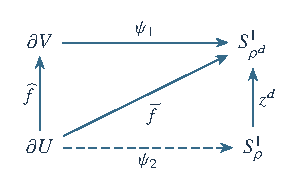
\includegraphics[width=.35\textwidth]{cd13-fig-01.pdf}
 \FigureTag{CD13.1}{fig:cd13-01}
\end{figure}
Since $\partial U,\partial V$ are analytic, $R$ and $f$ can be extended
analytically beyond $\partial U,\partial V$. Thus $\widetilde f$ remains
a branched covering of degree $d$, and we have
\[
 \widetilde f_*\bigl(\pi_1(\partial U)\bigr)
 \subseteq(z\mapsto z^d)_*\bigl(\pi_1(S^1_\rho)\bigr).
\]
Hence $\widetilde f$ can be lifted to $\psi_2$, giving
$\psi_1(f(z))=\psi_2(z)^d$ for every $z\in\partial U$.
Here $\psi_2\in\operatorname{Deck}(S^1_{\rho^d})$.
% Author check: the deck-group assertion and covering terminology are retained.
Let
\[
 A_0=V\setminus U,\qquad
 A_{\rho,\rho^d}:=\{\zeta:\rho<|\zeta|<\rho^d\}.
\]
The maps $\psi_1,\psi_2$ are analytic on $\partial V,\partial U$,
so there exists a quasiconformal map $\psi$ on $A_0$ such that
$\psi\colon\overline{A_0}\to A_{\rho,\rho^d}$ is continuous.
Now it is time to perform the surgery.
% Author check: A_0 and the target of its closure follow the source despite boundary inconsistencies.

% Source page 5
Tear off the domain of $f$ from its codomain, obtaining $V\setminus U$.
On this we have a quasiconformal map $\psi$. Let us use it to glue $f$
to a holomorphic map, which we shall later use as a hook to pull the
flattened circle field back to its original shape, that is, to straighten
an ellipse field to a circle field.
Define $F\colon\mathbb C\to\mathbb C$, the result of surgery on $f$, by
\[
 F(z):=
 \begin{cases}
  f(z),&z\in U,\\
  R^{-1}\bigl(\psi(z)^d\bigr),&z\in A_0,\\
  R^{-1}\bigl(R(z)^d\bigr),&z\in\mathbb C\setminus V.
 \end{cases}
\]
Note that $F$ is quasiregular. If we find an $F$-invariant Beltrami form,
the Mapping Theorem will conclude the proof.
Define the Beltrami form $\mu$ by
\[
 \mu(z):=
 \begin{cases}
  \psi^*\mu_0,&\text{on }A_0,\\
  R^*\mu_0,&\text{on }\mathbb C\setminus V,\\
  (f^n)^*\mu,&\text{on }\{z\in U:f^n(z)\in A_0\},\\
  \mu_0,&\text{elsewhere}.
 \end{cases}
\]
Clearly $\mu$ is $F$-invariant, so there exists a quasiconformal map
$\phi\colon\mathbb C\to\mathbb C$ such that
$\phi\circ F\circ\phi^{-1}$ is holomorphic on $\widetilde U=\phi(U)$,
of degree $d$.
% Source page 6
Therefore $F$ is quasiconformally conjugate to a holomorphic map;
in particular, $f$ is quasiconformally conjugate to a polynomial.
\end{proof}
% Author check: the pullback prescription and the global polynomial conclusion are abbreviated.

The theorem in fact says something more. Set
$K_f:=\bigcap_{n>0}f^{-n}(V)$.
Then $K_f$ is the right analogue of the filled Julia set for polynomials:
it is the set of points in $U$ that never escape $U$.
Note that $f$ and
$P=(\phi\circ F\circ\phi^{-1})|_{\phi(U)}$ are conjugate, but on $K_f$
they are conjugate holomorphically. Such a phenomenon is called
\emph{hybrid equivalence}.
% Author check: “holomorphically on K_f” is the source wording, not a supplied neighbourhood conjugacy.
% BLOG-CONTENT-END
\end{document}
